\documentclass[x11names, svgnames]{beamer}
\usepackage{listings}

\usetheme{sbi}

\title{Galaxy for linking bisulfite sequencing with RNA sequencing}
\author{Markus Wolfien, Andrea Bagnacani, Olaf Wolkenhauer}

\definecolor{Gray}{gray}{0.85}
\newcommand{\eg}{\textit{e}.\textit{g}.$\,\,$}

\begin{document}


%
% title
%
\frame[noframenumbering,plain]{\maketitle}



%
% outline
%
\newcommand{\one}{Who are we?}
\newcommand{\two}{Course outline}
\newcommand{\three}{RNA Sequencing (RNA-Seq)}
\newcommand{\four}{Next Generation Sequencing (NGS)}
\newcommand{\five}{Tools and materials}
\begin{frame}
  \frametitle{Outline}
  \begin{itemize}
    \itemsep1em
    \item \one
    \item \two
    \item \three
    \item \four
    \item \five
  \end{itemize}
\end{frame}



%
%
%
\begin{frame}
  \frametitle{\one}
  \begin{center}
    
\includegraphics[scale=0.15]{images/people_denbi}
  \end{center}
  \begin{center}
    \footnotesize{\href{https://denbi.de}{\textcolor{gray}{https://denbi.de}}}
  \end{center}
  \begin{center}
    \small{
  The \textit{German Network for Bioinformatics Infrastructure} - \textbf{de.NBI} consists of eight service units that provide distinct bioinformatics services according to their areas of scientific expertise and their bioinformatics resources. The units complement each other in terms of thematic priorities, implementing user services in different areas of Life Sciences research and in industry. The services are complemented by comprehensive training activities.}
  \end{center}
\end{frame}
\begin{frame}
  \frametitle{\one}
  \begin{center}
    
\includegraphics[scale=0.3]{images/logo_destair}
  \end{center}
  \begin{center}
    \footnotesize{\href{https://destair.bioinf.uni-leipzig.de}{\textcolor{gray}{https://destair.bioinf.uni-leipzig.de}}}
  \end{center}
  \begin{center}
    \vspace{2em}
    \small{
    The \textit{Structured Analysis and Integration of RNA-Seq experiments} - \textbf{de.STAIR} provides comprehensive analyses of RNA-Seq experiments as a service. To bring ease of use, reproducibility, and accessibility for the developed approaches and services, we provide dedicated workshops, training programs and screen casts for bioinformaticians and other life scientists.}
  \end{center}
\end{frame}
\begin{frame}
  \frametitle{\one}
  \begin{center}
    Who are you? :)
  \end{center}
\end{frame}



%
%
%
\begin{frame}
  \frametitle{\two}
  \begin{center}
    
\includegraphics[scale=0.1]{images/logo_github}
  \end{center}
  \begin{center}
    \footnotesize{\href{https://github.com/destairdenbi/trainings}{\textcolor{gray}{https://github.com/destairdenbi/trainings}}}
  \end{center}
\end{frame}



%
%
%
\begin{frame}
  \frametitle{\three}
  \begin{center}
  RNA-Seq is able to identify thousands of differentially expressed genes, tens of thousands of differentially expressed gene isoforms and can detect mutations and germline variations for hundreds to thousands of expressed genetic variants, as well as detecting chimeric gene fusions, transcript isoforms and splice variants.
  \end{center}
  \begin{center}
    \vspace{2em}
    \footnotesize{\href{https://doi.org/10.1038/nrg2484}{\textcolor{gray}{Wang, Nature 2009}}}
  \end{center}
\end{frame}
\begin{frame}
  \frametitle{\three}
  \begin{center}
    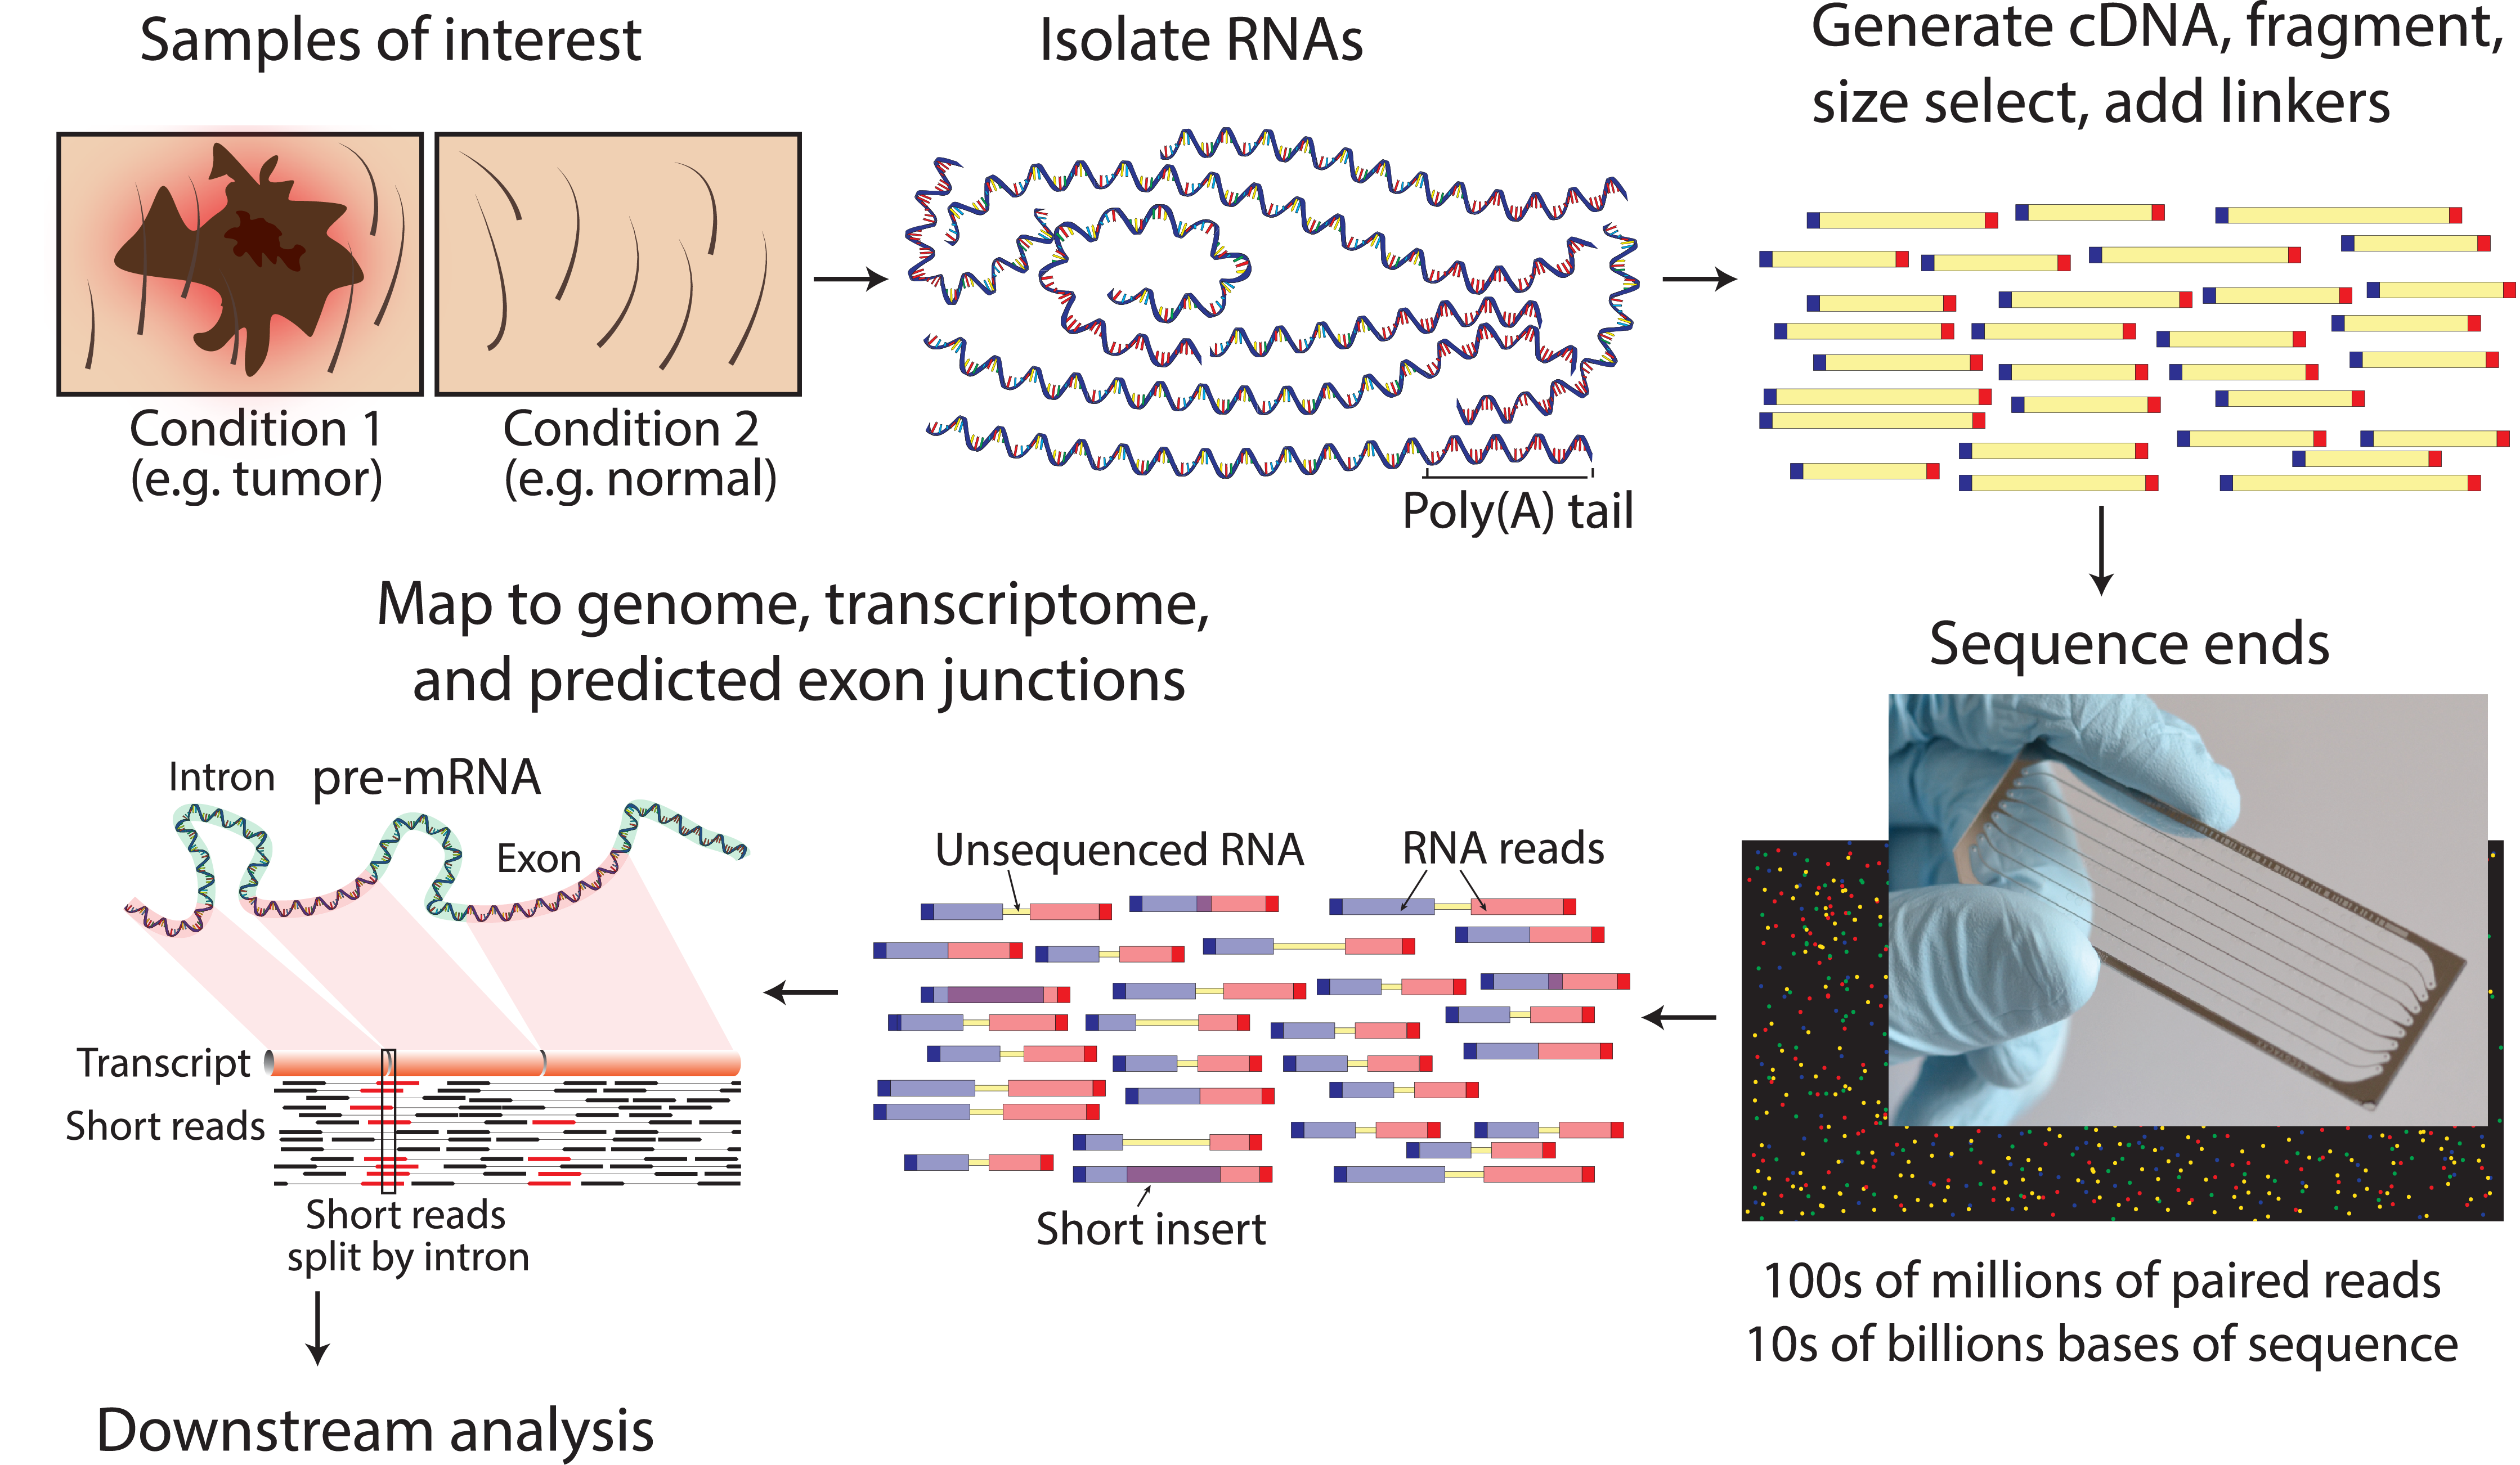
\includegraphics[scale=0.55]{images/griffith-plos}
  \end{center}
  \begin{center}
    \vspace{1.5em}
    \footnotesize{\href{https://doi.org/10.1371/journal.pcbi.1004393}{\textcolor{gray}{Griffith et al., PLOS 2015}}}
  \end{center}
\end{frame}



%
%
%
\begin{frame}
  \frametitle{\four}
  \begin{columns}[T]
    \begin{column}{0.5\textwidth}
      \begin{center}
        \vspace{-2em}
        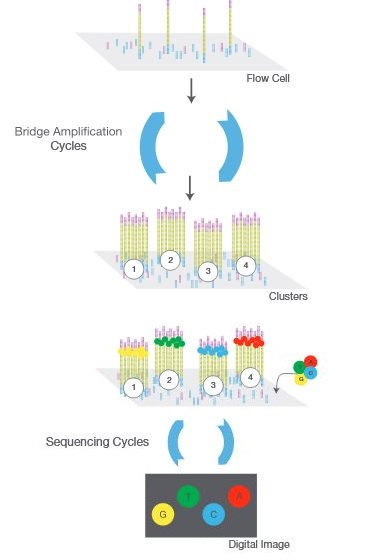
\includegraphics[scale=0.55]{images/illumina_sequencing}
      \end{center}
    \end{column}
    \begin{column}{0.5\textwidth}
      \begin{center}
        \vspace{-1em}
        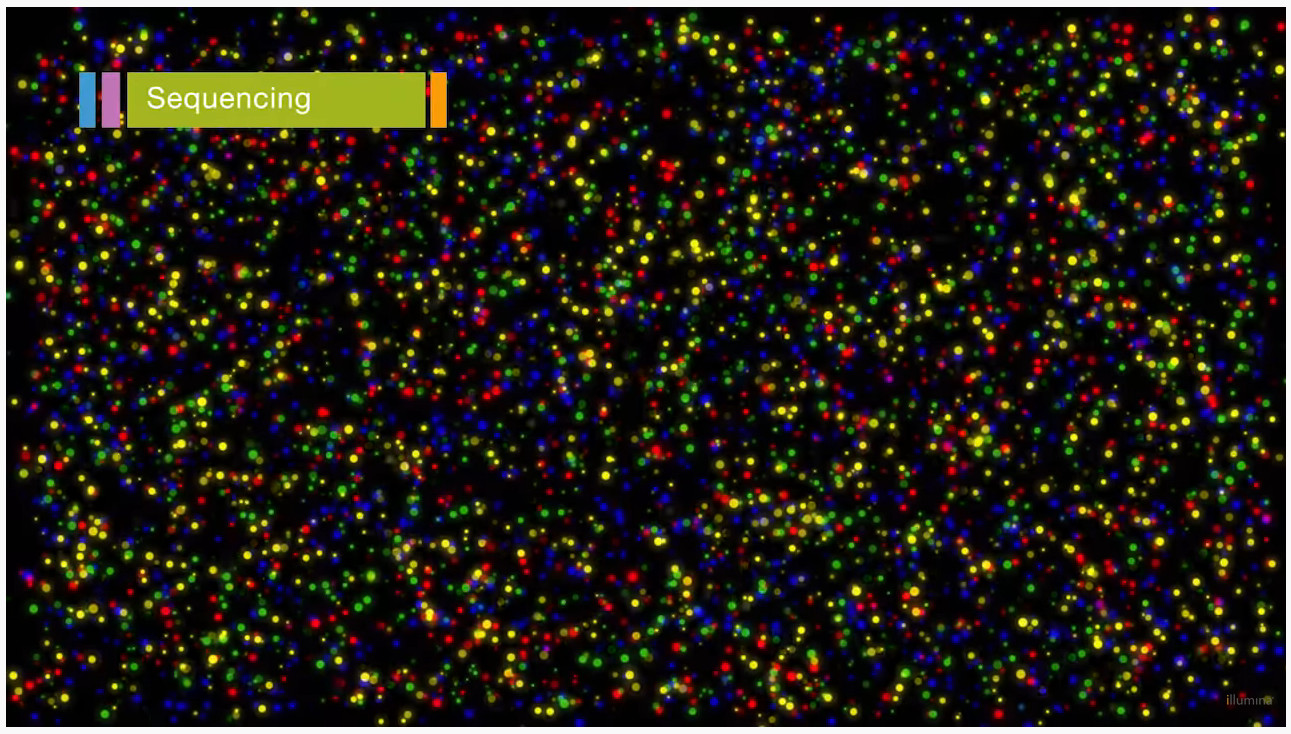
\includegraphics[scale=0.15]{images/illumina_video}
      \end{center}
      \begin{center}
        \tiny{\href{https://www.youtube.com/watch?v=fCd6B5HRaZ8}{\textcolor{gray}{https://www.youtube.com/watch?v=fCd6B5HRaZ8}}}
      \end{center}
      \vspace{4em}
      \footnotesize{
        \hfill\href{https://www.well.ox.ac.uk/ogc/sequencing-quality-monitoring-run/}{\textcolor{gray}{Oxford Genomics Centre, 2017}}
      }
      \vspace{6em}
      \footnotesize{
        \hfill\href{https://emea.illumina.com/content/dam/illumina-marketing/documents/products/other/ivf-reproductive-genetic-health-ngs-primer-1570-2015-012.pdf}{\textcolor{gray}{Illumina, 2015}}
      }
    \end{column}
  \end{columns}
\end{frame}
\begin{frame}
  \frametitle{\four}
  The decrease of sequencing costs is met with an increased effort in data processing $\implies$ Increased need of Bioinformatics expertise.
  \begin{center}
    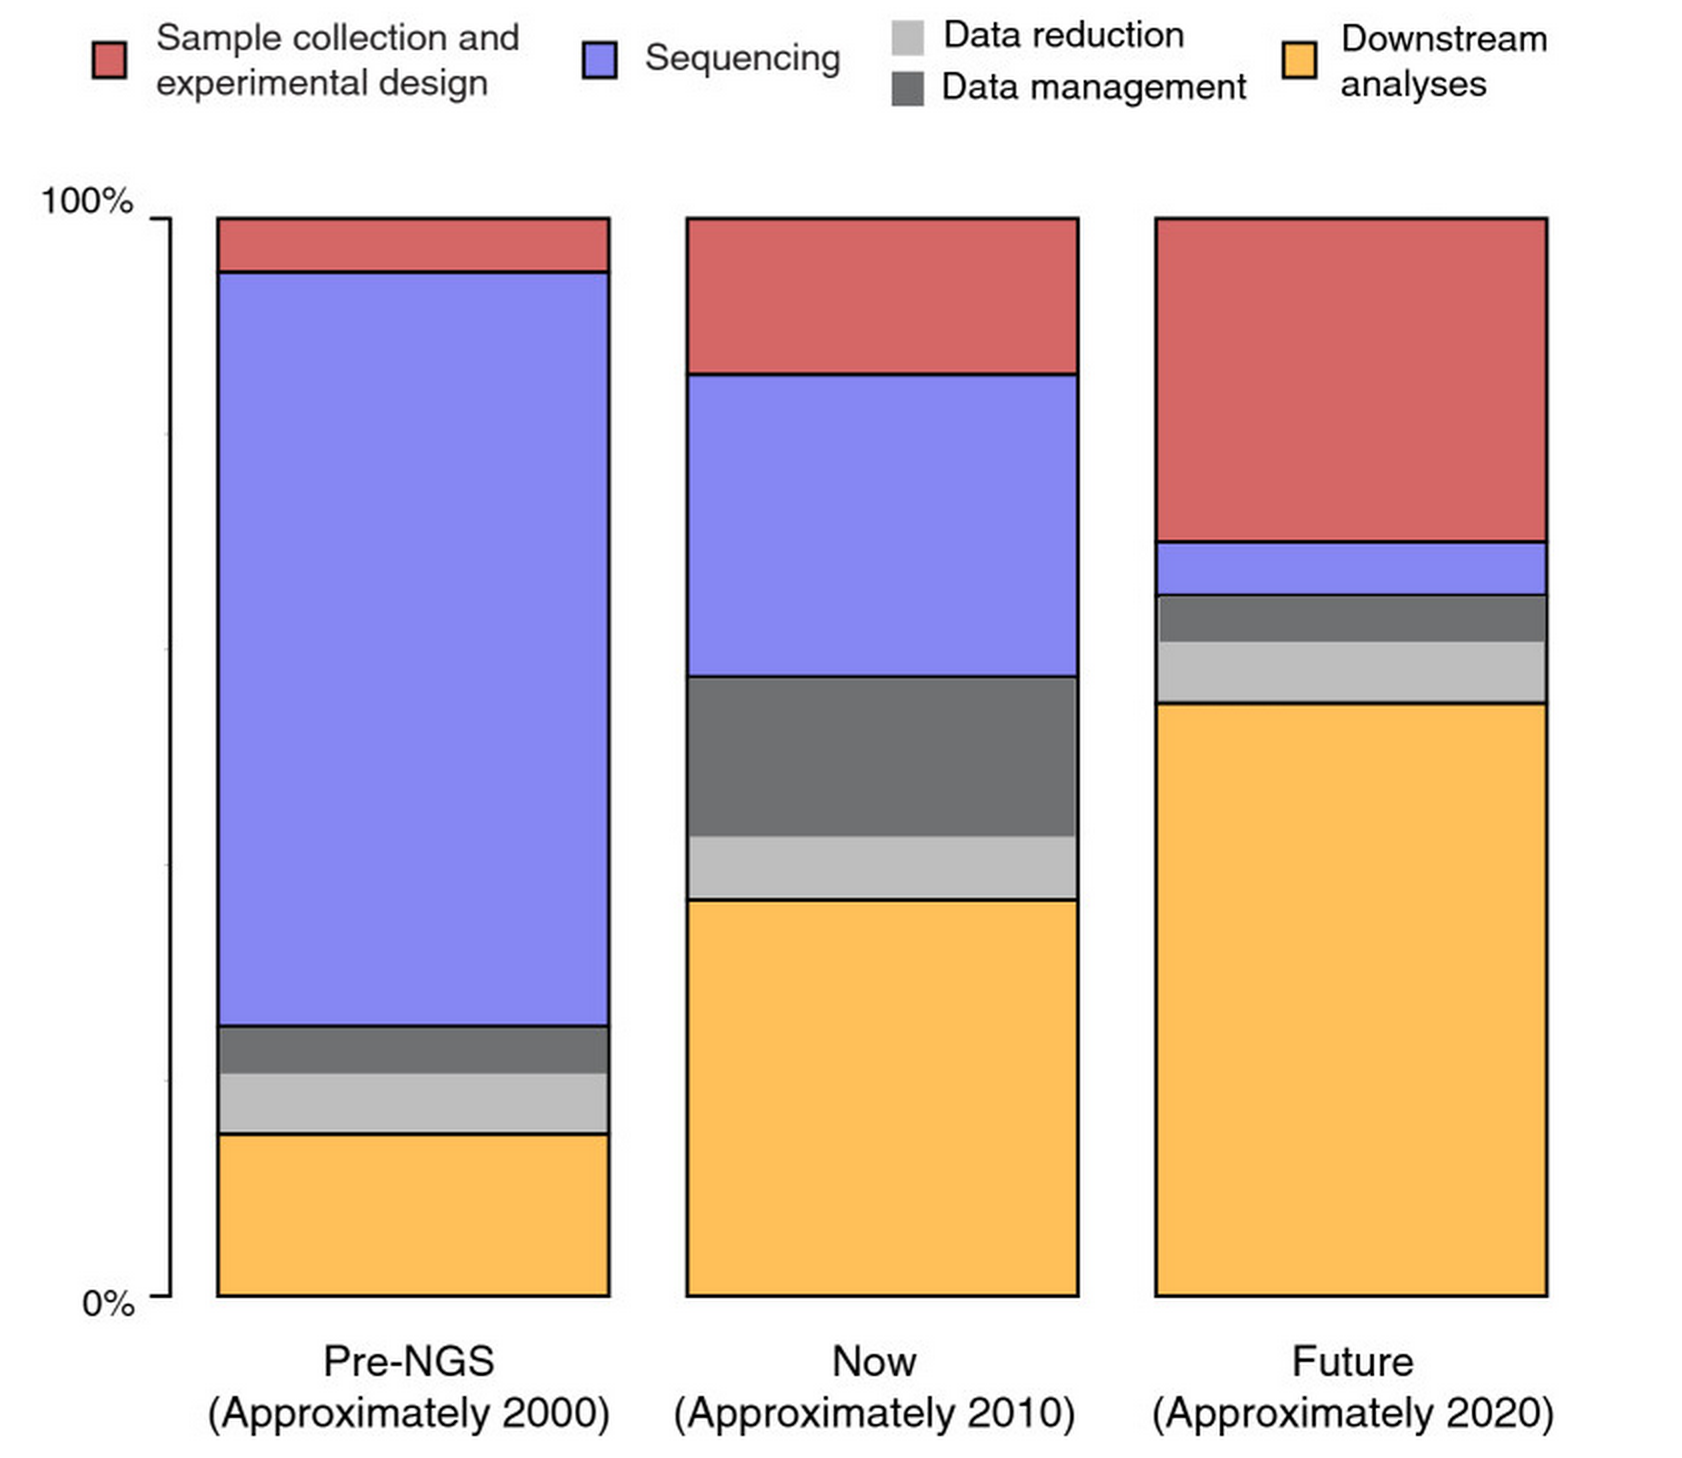
\includegraphics[scale=0.11]{images/sequencing_cost}
  \end{center}
  \begin{center}
    \vspace{-0.5em}
    \footnotesize{\href{https://doi.org/10.1186/gb-2011-12-8-125}{\textcolor{gray}{Sboner et al., Genome Biology 2011}}}
  \end{center}
\end{frame}



%
%
%
\begin{frame}
  \frametitle{\five}
  \begin{center}
    \vspace{-1em}
    
\includegraphics[scale=0.11]{images/logo_galaxy}
  \end{center}
  \begin{center}
    \footnotesize{\href{https://usegalaxy.eu}{\textcolor{gray}{https://usegalaxy.eu}}}
  \end{center}
  \begin{center}
    \vspace{2em}
    
\includegraphics[scale=0.11]{images/logo_gtn}
  \end{center}
  \begin{center}
    \footnotesize{\href{https://galaxyproject.github.io/training-material/}{\textcolor{gray}{https://galaxyproject.github.io/training-material/}}}
  \end{center}
\end{frame}

\end{document}
